\chapter{System Description}
A surface vessel is provided for the project, \cite{aauship}. As seen in \autoref{fig:systemphoto} the boat is equipped with actuators, sensors and control electronics.

\begin{figure}[H]
    \includegraphics[width=.65\textwidth]{figures/system}
    \caption{System picture. The arrows point to the components used in the project.}
    \label{fig:systemphoto}
\end{figure}

The surface vessel at hand is a complex system composed by several subsystems. These are shown in \autoref{fig:systemDiagram}, in which the link between the different subsystems is also depicted.
%
\begin{figure}[H]
    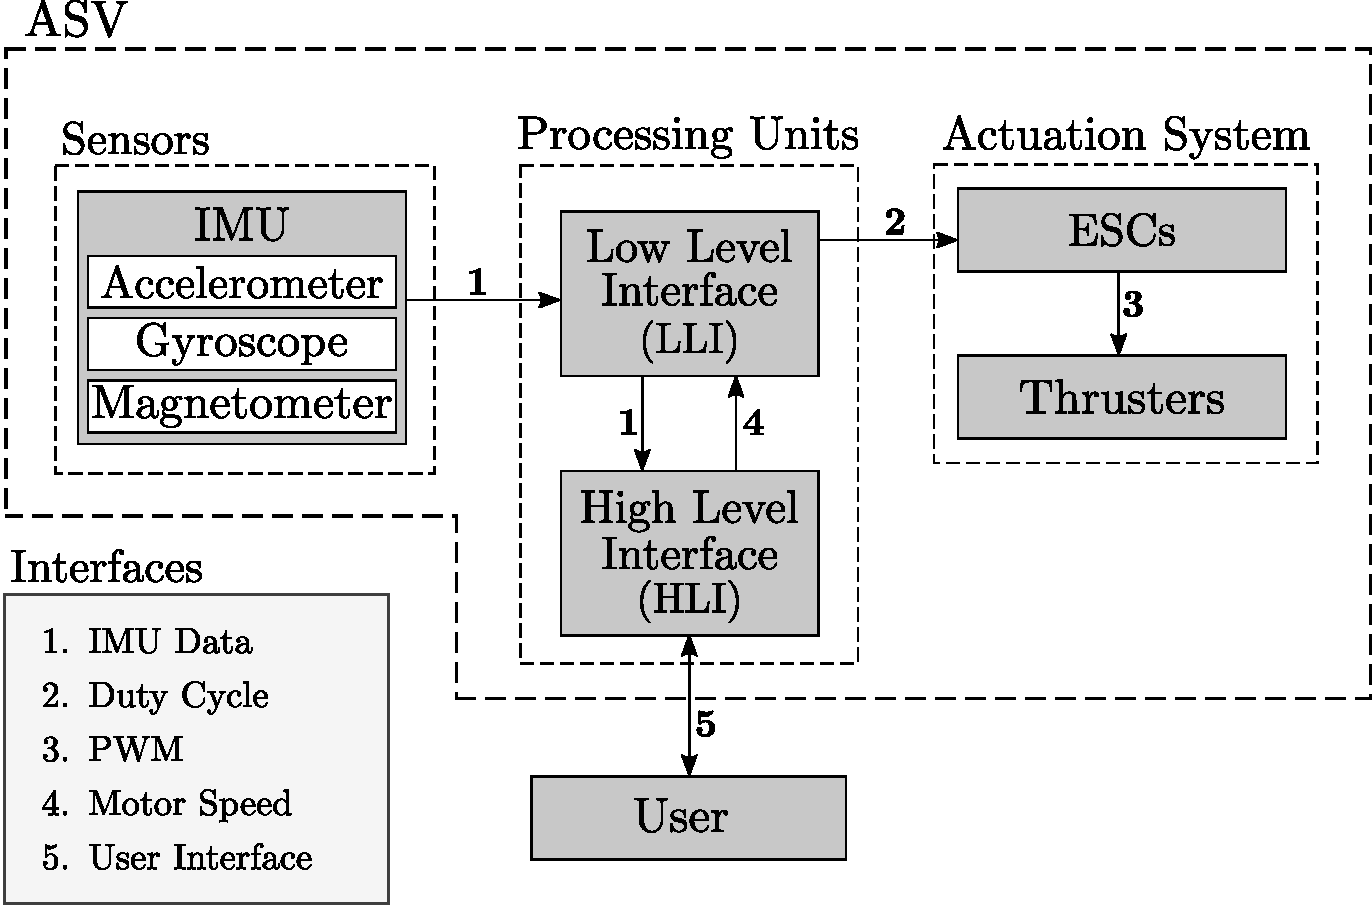
\includegraphics[width=.65\textwidth]{figures/systemDiagram4}
    \caption{Functional diagram of the given system.}
    \label{fig:systemDiagram}
\end{figure}
%
%The main parts of the system are the actuation system, the sensors and the processing units, see \autoref{fig:systemDiagram}. The processing unit gathers information from the IMU. This is handled by the Low Level Interface (LLI) which then sends it to the High Level Interface (HLI) where the control algorithms are implemented. The calculated actuation is then sent back to the LLI that sends the command to the actuation system. The ESCs (electronic speed controllers) then calculate the required signal to make the motors turn at the requested speed.

The main parts of the system are the actuation system, the sensors and the processing units, see \autoref{fig:systemDiagram}. The inertial measurement unit (IMU) information is gathered by the low level interface (LLI), and then transferred to the high level interface (HLI). In the HLI, the control algorithms are implemented, and the calculated commands are sent back to the actuation system through the LLI. The electronic speed controllers (ESCs) then calculate the required signal to make the motors turn at the requested speed.

This chapter briefly describes the main components of the surface vessel used in this project. Some additions to the existing systems are also presented.

